\documentclass[]{llncs}
\usepackage{graphicx}

%\documentclass{article}
\usepackage{mathtools}
\usepackage{times}  % DO NOT CHANGE THIS
\usepackage{helvet} % DO NOT CHANGE THIS
\usepackage{courier}  % DO NOT CHANGE THIS
\usepackage[hyphens]{url}  % DO NOT CHANGE THIS
\usepackage{arydshln}
\usepackage{mathptmx}
\usepackage{amsmath}
\usepackage{bm}
\usepackage[english]{babel}
\usepackage[utf8]{inputenc}
\usepackage{algorithm}
\usepackage{epstopdf}
\usepackage{booktabs}
\usepackage{multirow}
\usepackage{siunitx}
\usepackage{rotating}
\usepackage{hyperref}
\usepackage[utf8]{inputenc}
\usepackage[T1]{fontenc}
\usepackage{mathtools}
\usepackage[thinc]{esdiff}
%\usepackage[algo2e]{algorithm2e}
%\usepackage{arevmath}     % For math symbols
\usepackage[noend]{algpseudocode}
\urlstyle{rm} % DO NOT CHANGE THIS
\def\UrlFont{\rm}  % DO NOT CHANGE T
% Used for displaying a sample figure. If possible, figure files should
% be included in EPS format.
%
% If you use the hyperref package, please uncomment the following line
% to display URLs in blue roman font according to Springer's eBook style:
% \renewcommand\UrlFont{\color{blue}\rmfamily}

\pagestyle{plain}
\setcounter{page}{1}
\pagenumbering{arabic}

\DeclareMathOperator {\argmax}{argmax} 

\begin{document}

\title{Adaptive Dynamics for the Direct Actions Strategy Approach}

\author{Frances Cameron-Muller, Supervisor: Dr. Julian Garcia}

\institute{Monash University}

\maketitle    

\section{Basic Model}

\subsection{Adaptive Dynamics Analysis}

The model consists of a population of agents that are matched into pairs to play a Stag Hunt game. Let $x_i \in [0,1]$ be the probability that agent i cooperates with their matched opponent. \\
The Stag Hunt Payoff Matrix is 
\[
  \begin{pmatrix} 
   R & S  \\
   T & P  
   \end{pmatrix} 
\]
with $ R > T \geq P > S. $ \\
\\
Let $ \Pi ( y, x_{-} )$ be the payoff function of playing a strategy y against the rest of the population playing the strategy x. The payoff function $ \Pi ( y, x_{-} )$ measures the expected reward of an agent playing strategy y against opponents playing the strategy x. 
\[
\Pi ( y, x_{-} ) = R x y + S (1-x) y +  T x (1-y) + P (1-x) (1-y)
\]
\\
The initial growth rate of a mutant strategy is known as its invasion fitness, a quantity that describes the likelihood of the mutant strategy surviving in the population. A positive invasion fitness means the mutant strategy has a positive probability of surviving and a negative invasion fitness means the mutant strategy will more likely go extinct. In this model, the invasion fitness of a rare mutant strategy y in a population with a dominant strategy x is measured by the difference in the payoff functions of the mutant strategy against the dominant strategy and the payoff function of the dominant strategy against itself. 
\[
f_x(y) = \Pi ( y, x_{-} ) - \Pi ( x, x_{-} )
\]
\begin{multline}
f_x(y) = R x y + S (1-x) y +  T x (1-y) + P (1-x) (1-y) \\ - R x^2 - S (1-x) x - T x (1-x) - P (1-x) (1-x)
\end{multline}
\\
The derivative of invasion fitness evaluated at the point of the dominant strategy is known as the selection gradient and determines the direction of evolutionary change. If the selection gradient is positive then mutant strategies with slightly higher values are more likely to invade and vice-versa. 
\[
D(x) = \diffp*{f_x(y)}{y}{y=x}
\]
\[
D(x) = (R - S - T +P) x + (S-P)
\]
\\
Points where the selection gradient vanishes are known as evolutionarily singular strategies. These are significant points as this is where evolutionary stable strategies or evolutionary branching may occur. A evolutionary singular point is only an evolutionary stable point if the second derivative of the invasion fitness at that point is negative. 
\[
D(H) = 0
\]
\[H = \frac{P-S}{R - S - T +P} 
\]
\\
For $x < H, D(x) < 0$ and for $x > H, D(x) > 0.$ This means that for beliefs below the threshold, the best payoffs are achieved by decreasing the value of the belief (cooperating less) and converging to the Nash equilibrium of always defecting. For beliefs above the threshold, the best payoffs are achieved by increasing the value of the belief and converging to the Nash equilibrium of always cooperating. 

\subsection{Graphs}

Figure 1 below plots the invasion fitness function for all the values the mutant strategy can take against different dominant strategies. This graph shows, given a population with dominant strategy x, which mutant strategy values will have a positive invasion fitness and successfully invade. The payoff matrix of this game is [4,1;3,2] with a threshold H = 0.5. This graph illustrates that when the dominant strategy is less than the threshold, mutant strategies with values less than the dominant strategy will survive and the game will converge to the defect-defect equilibrium. However, when the dominant strategy is greater than the threshold, mutant strategies greater than the dominant strategy will survive and the game will converge to the cooperate-cooperate equilibrium. Overall, the direction of evolutionary change depends if the dominant strategy is above or below the threshold. \\

\begin{figure}
\centering
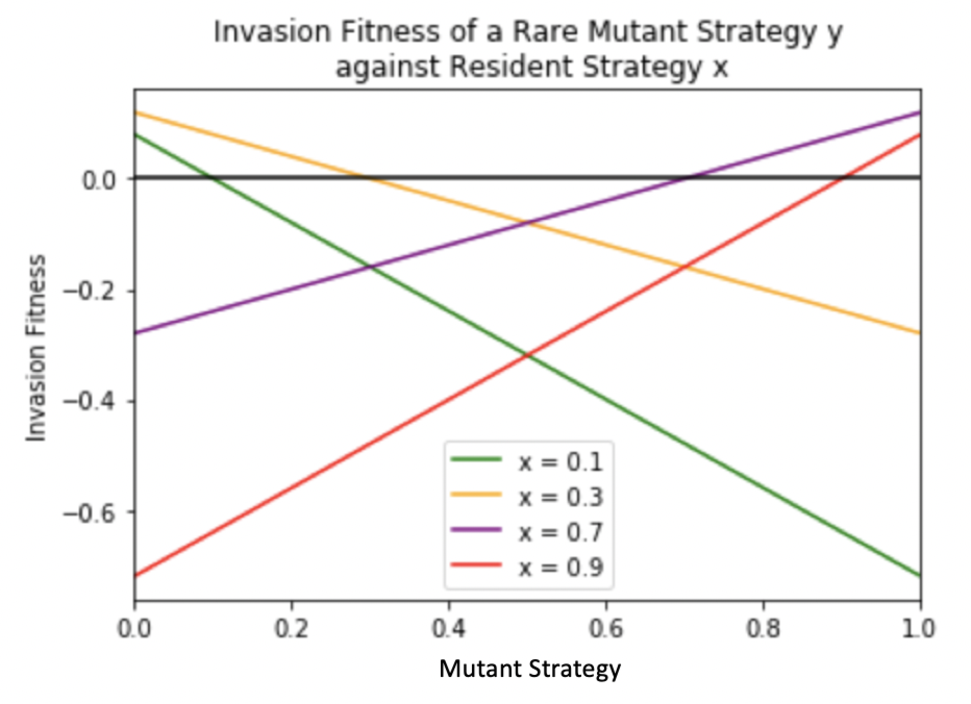
\includegraphics[width=12cm]{images/inv_fit_basic}
\caption{ }
\end{figure}

Pairwise invasibility plots (PIP) are graphs that plot the sign of the invasion fitness for all possible pairings of dominant and mutant strategies. They are visual tools that illustrate which combinations will result in successful invasion of the mutant strategy. Figure 2 below shows the PIP graphs for two payoff matrices. The green shaded areas indicates areas where invasion has a positive probability and the intersection of green areas indicate evolutionary singular strategies. The difference in the two PIP graphs show that for the second matrix with a lower threshold H = 0.25, there is more green area above the threshold that can lead to converging to social cooperation and less area in the green area that leads to the defecting equilibrium. 

\begin{figure}
\centering
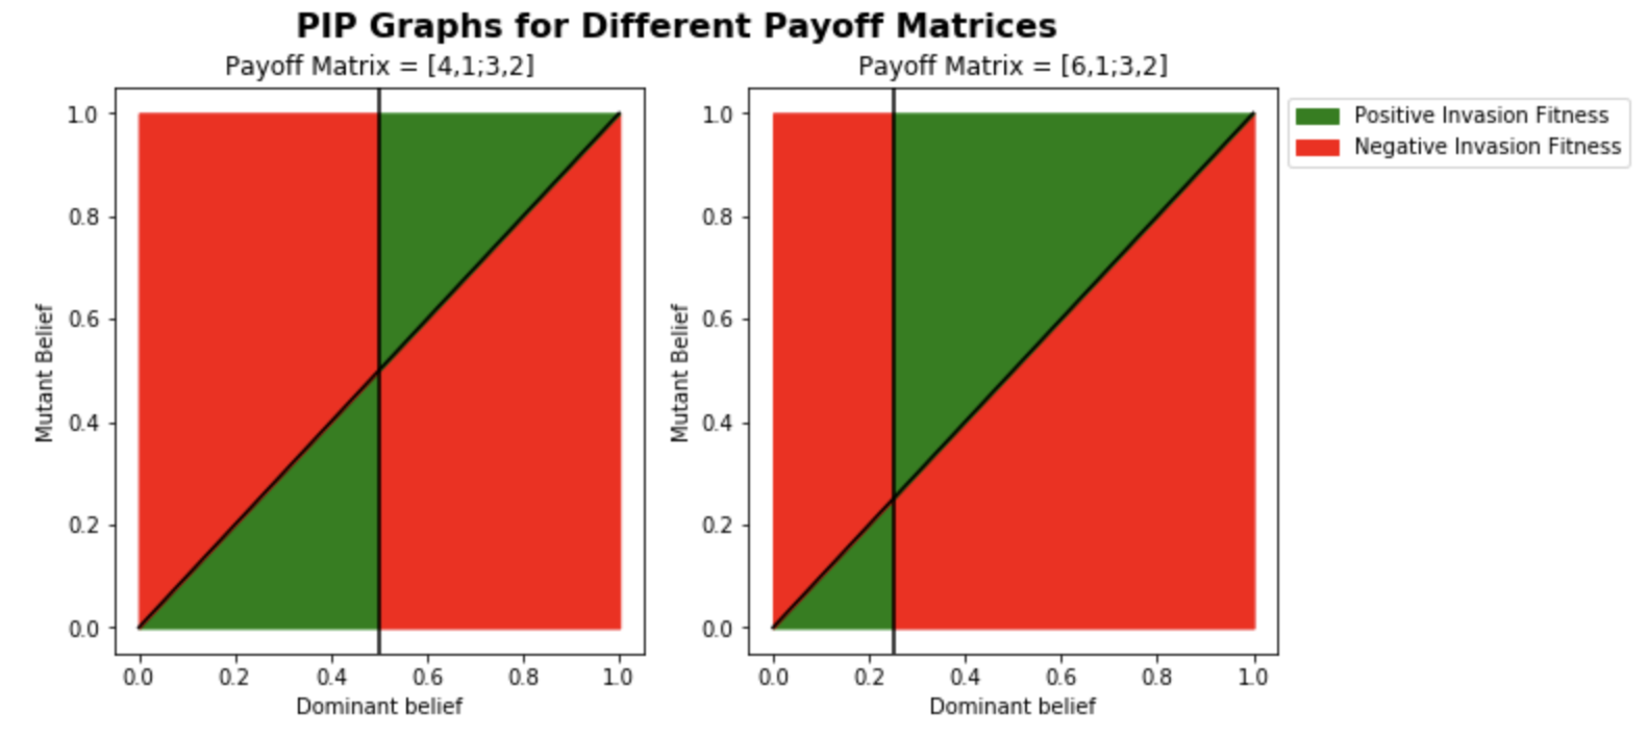
\includegraphics[width=15cm]{images/pip_basic}
\caption{ }
\end{figure}


\section{Alpha Model}

\subsection{Adaptive Dynamics Analysis}

To extend the model to account for population structure, we introduce a new parameter $\alpha \in [0, 1]$ where $\alpha$ is the probability that an agent is matched to play against a copy of themselves instead of their original opponent. Therefore, the new payoff function is given by the sum of payoffs of when an agent plays their copy and when an agent plays their original opponent, weighted by the probabilities.
\[ 
\Pi ( y, x_{-}, \alpha ) = \alpha \Pi ( y, y) + (1-\alpha) \Pi ( y, x_{-} )
\]
The new invasion fitness of a rare mutant strategy y in a population with a dominant strategy x is given by 
\[
f_x(y) = \Pi ( y, x_{-}, \alpha ) - \Pi ( x, x_{-}, \alpha )
\]
\[
f_x(y) = \alpha \Pi ( y, y) + (1-\alpha) \Pi ( y, x_{-} ) - \alpha \Pi ( x, x) - (1-\alpha) \Pi ( x,  x_{-} )
\]
\[
f_x(y) = \alpha \Pi ( y, y) + (1-\alpha) \Pi ( y, x_{-} ) - \Pi ( x,  x_{-} )
\]
\begin{multline}
f_x(y) = \alpha (R-S-T+P) y^2 +(S + \alpha T - P - \alpha P) y + (1-\alpha) (R-S-T+P) x y \\+ (-\alpha T + \alpha P - S + P) x + (-R+S+T-P) x^2
\end{multline}
The selection gradient and evolutionarily singular strategies for the alpha model are given by 
\[
D(x) = \diffp*{f_x(y)}{y}{y=x}
\]
\[
D(x) = (1+\alpha) (R-S-T+P) x + (S + \alpha T - P - \alpha P) 
\]
\[
D(H) = 0
\]
\[
H = \frac{-S - \alpha T + P + \alpha P}{(1+\alpha)(R-S-T+P)}
\]

\subsection{Graphs}

Figure 3 shows the selection gradient of a mutant strategy, D(x), for three values of alpha using the payoff matrix [4,1;3,2]. When alpha = 0, meaning the  probability that an agent is matched to play against a copy of themselves instead of their original opponent is zero, we observe the same function of the basic model. When alpha = 1, D(x) is always positive, illustrating that the agents will always learn to cooperate if they are only playing against a copy of themselves. For alpha values between 0 and 1, as alpha increases the threshold for D(x) decreases. Therefore, the more likely the agents are to play against opponents that are similar to themselves, the more likely they will learn to cooperate. This conclusion is supported by Figure 4 that plots invasion fitness against mutant strategy values for different values of alpha and dominant strategies. 

\begin{figure}
\centering
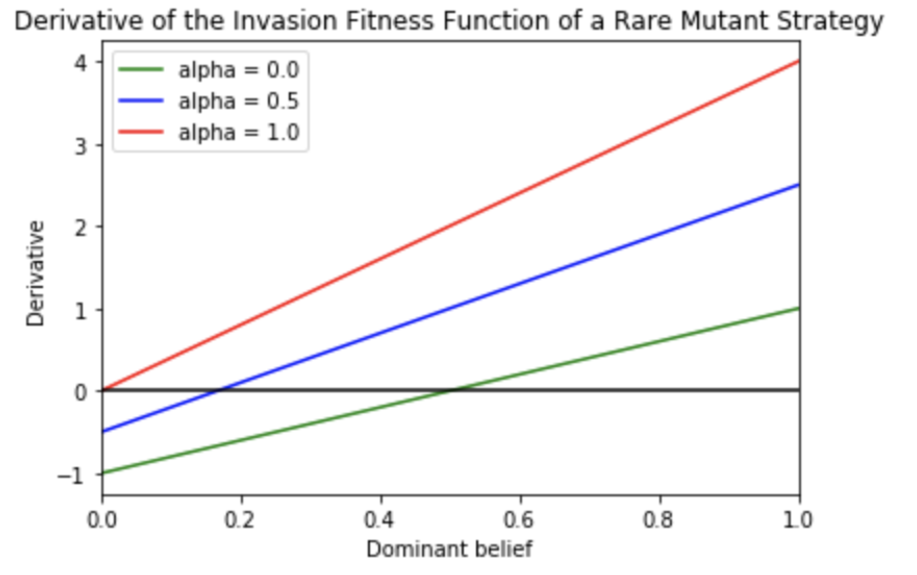
\includegraphics[width=12cm]{images/invasion_fitness_alpha}
\caption{ }
\end{figure}

\begin{figure}
\centering
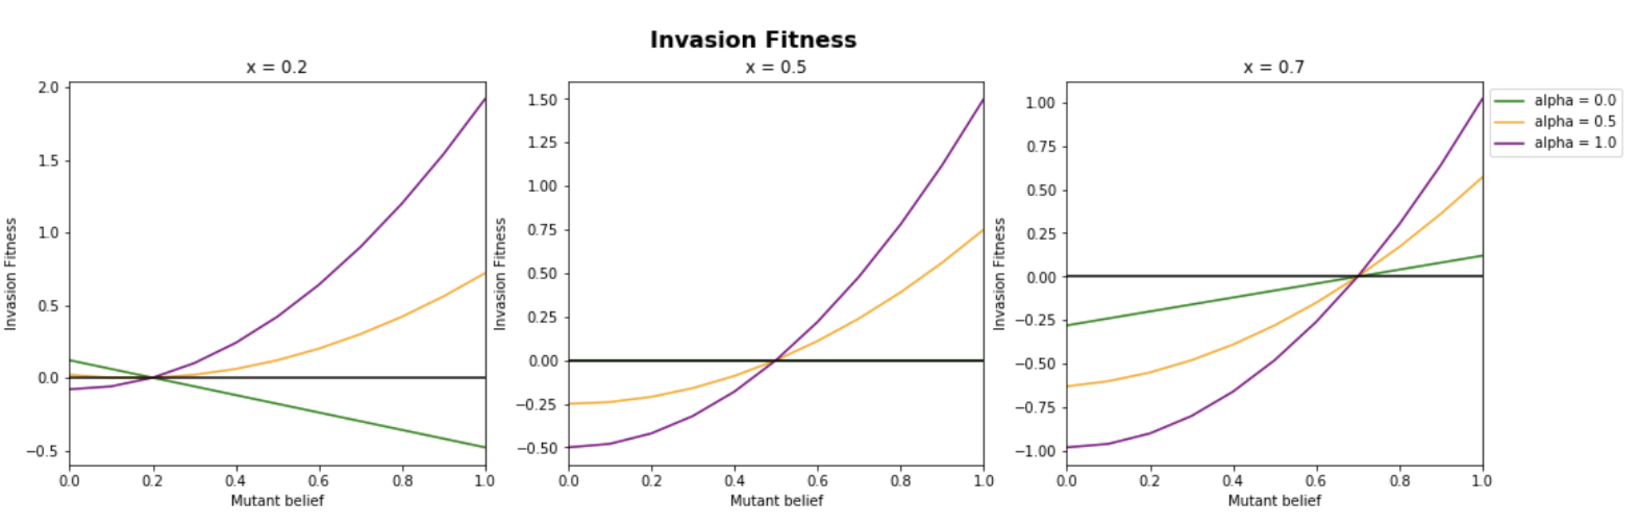
\includegraphics[width=15cm]{images/inv_fit_alpha}
\caption{ }
\end{figure}

PIP graphs for three values of alpha are shown below in Figure 5 and illustrate that as alpha increases, the number of combinations of mutant and dominant strategies that have a positive invasion fitness increases. 

\begin{figure}
\centering
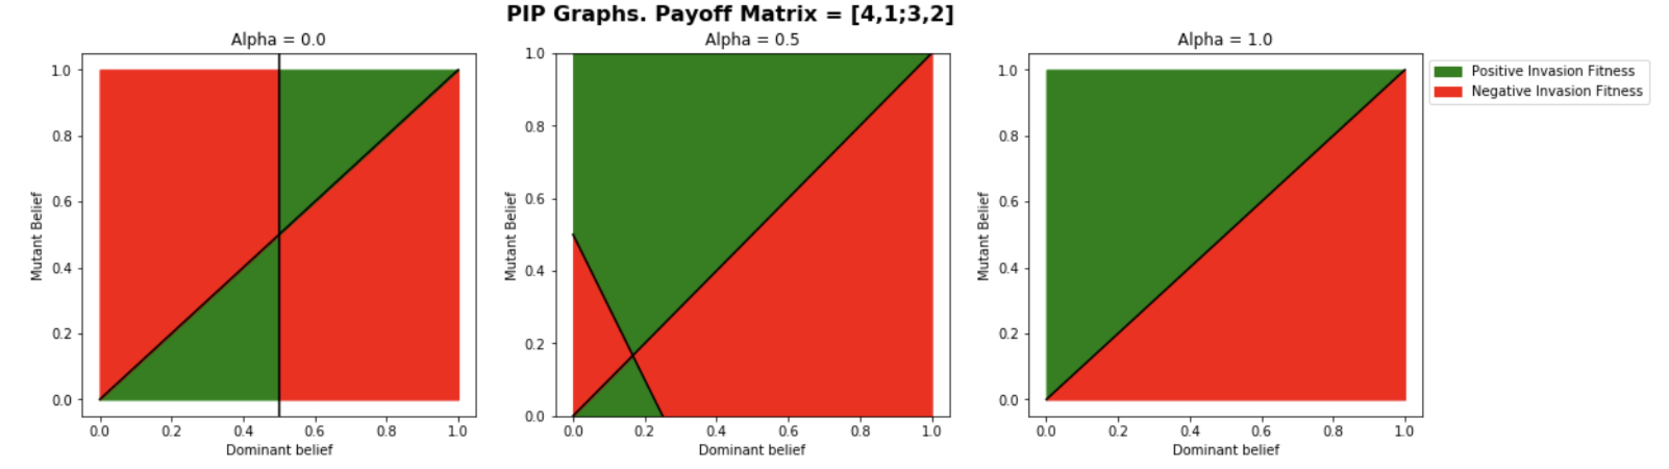
\includegraphics[width=15cm]{images/pip_alpha}
\caption{ }
\end{figure}

\section{Beta Model}

\subsection{Adaptive Dynamics Analysis}

In the beta model, each agent in the population has a two-dimensional strategy profile strategy, $x_i$, consisting of an ingroup and outgroup strategy,  $x_i = (x_{in}, x_{out})$\\
\\
Let $x_{in} \in [0,1]$ be the probability that an agent with a strategy profile x cooperates with an individual from the ingroup. \\
\\
Let $x_{out} \in [0,1]$ be the probability that an agent with a strategy profile x cooperates with an individual from the outgroup. \\
\\
Let $\beta_i \in [0,1]$ be the probability that agent i plays an individual from the ingroup.\\
\\
Let $\beta_{-i} = 1 -\beta_i $ be the probability that an agent of the opposite group of agent i plays an individual from the ingroup.\\
\\
Let $ \Pi ( y, x_{-}, \beta_y)$ be the payoff function of playing a strategy $y = (y_{in}, y_{out}) $ against the rest of the population playing the strategy $x = (x_{in}, x_{out})$ where the probability of an agent playing the strategy y matching with an individual from the ingroup is $\beta_y$.
\[
\Pi ( y, x_{-} , \beta_y) = \beta_y \Pi ( y_{in}, x_{in}) + (1-\beta_y) \Pi ( y_{out}, x_{out} ) 
\]
\\
The invasion fitness of a rare mutant strategy y in a population with a dominant strategy x is given by 
\[
f_x(y) = \Pi ( y, x_{-} , \beta_y) - \Pi ( x, x_{-} , \beta_x) 
\]
where $\beta_x = 1 - \beta_y.$
\[
f_x(y) = \beta_y \Pi ( y_{in}, x_{in}) + (1-\beta_y) \Pi ( y_{out}, x_{out} )  - \beta_x \Pi ( x_{in}, x_{in}) - (1-\beta_x) \Pi ( x_{out}, x_{out} ) 
\]
\\
The selection gradient and the evolutionarily singular strategies for the beta model are given by 
\[
D(x) = \diffp*{f_x(y)}{y}{y=x}
\]
\[
D(x) = (\beta_y((R - S - T + P) x_{in} + (S-P)), (1-\beta_y)((R - S - T + P) x_{out} + (S-P)))
\]
\[
D(H) = 0 
\]
\[
H = (\frac{P-S}{\beta_y((R - S - T + P) }, \frac{P-S}{(1-\beta_y)((R - S - T + P) }) 
\]
\\
For the beta model, D(x) can have partial derivatives that are negative, positive or zero in any combination. The first partial derivative describes how the agent should modify their ingroup strategy and the second partial derivative describes how the agent should adjust their outgroup strategy. 


\subsection{Graphs}
The selection gradient function of a mutant strategy with respect to the ingroup and outgroup strategy is graphed below in Figure 6. Negative values of the selection gradient indicate the best payoffs are achieved by decreasing the value of strategy whereas for positive values of $D(x)$, greater payoffs are achieved by increasing the strategy. The selection gradients are graphed for three different values of $\beta$. The left graph shows that as the probability of an agent plays an individual from the ingroup increases, meaning they belong to an increasing majority, the absolute value of $D(x_{in})$ increases. Whereas, the right graph illustrates that the opposite behaviour is observed for the selection gradient with respect to the outgroup. This result can be interpreted as when the agent belongs to a larger group within the population they update their strategies more rapidly. \\

\begin{figure}
\centering
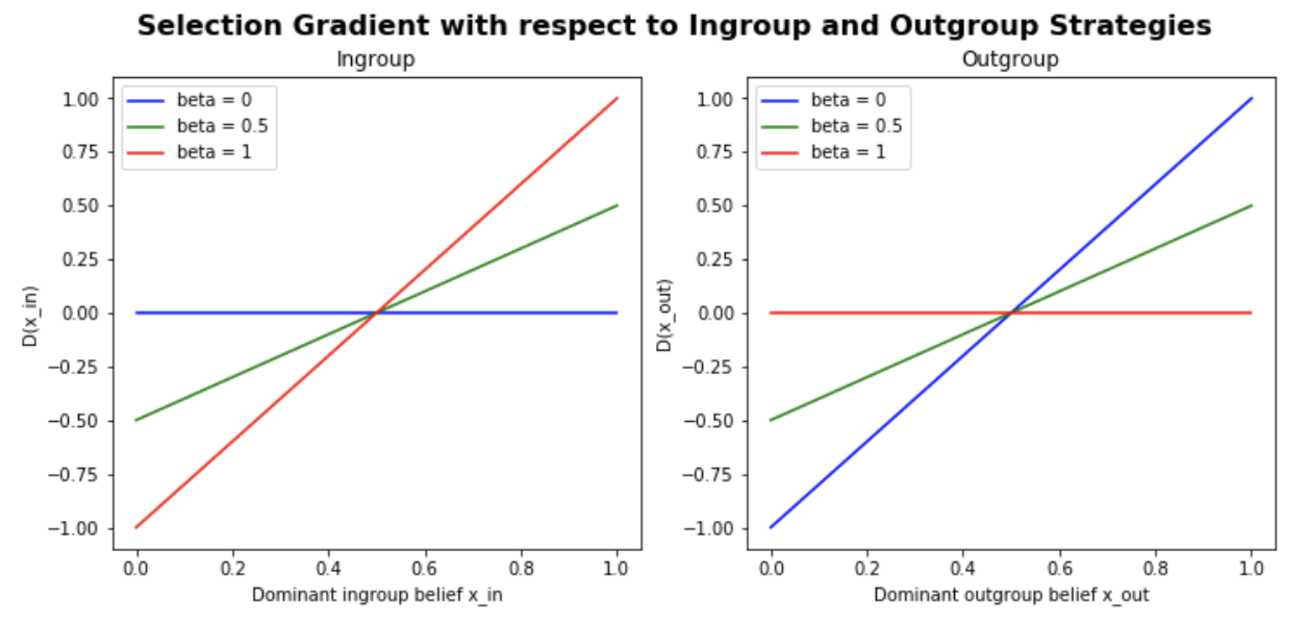
\includegraphics[width=12cm]{images/beta_sg}
\caption{ }
\end{figure}

The invasion fitness for all combinations of mutant ingroup and outgroup strategies against the dominant strategy (0.9,0.1) is graphed in Figure 7 for various beta values. This graph illustrates an example of how beta effects the invasion fitness of possible 2-dimensional mutant strategies.

\begin{figure}
\centering
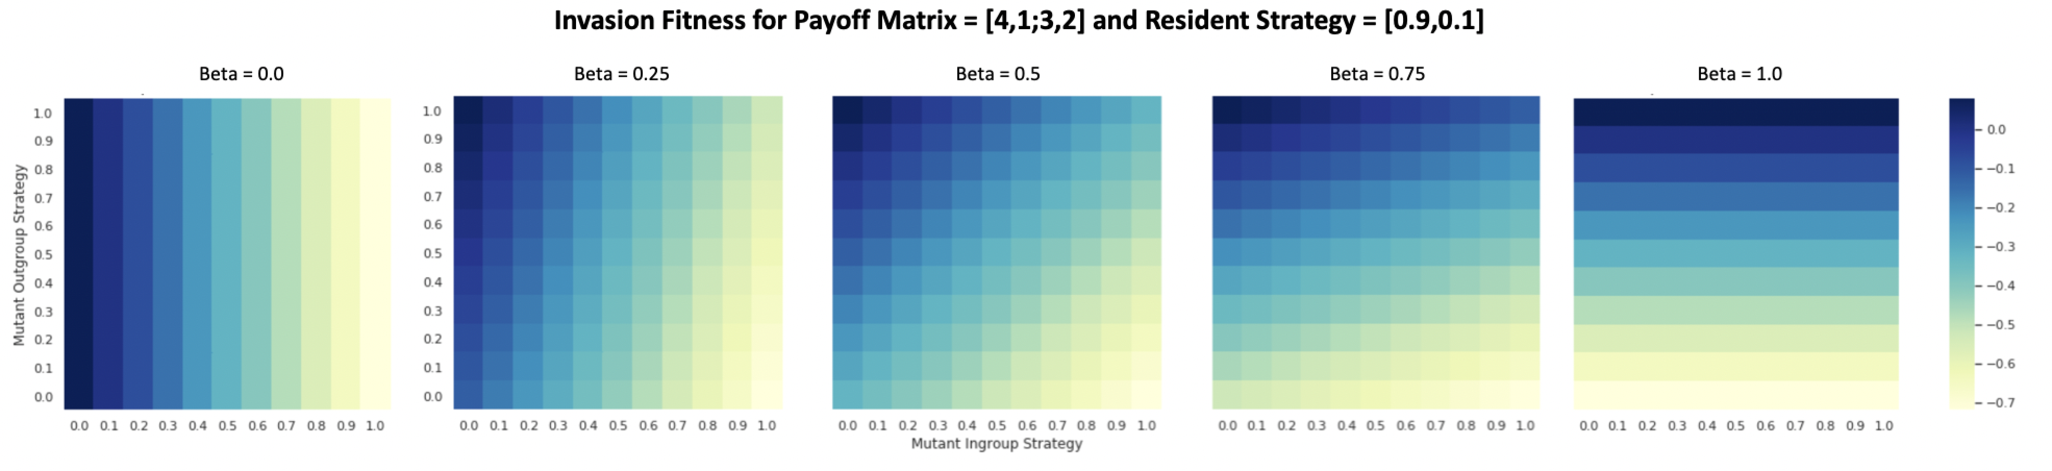
\includegraphics[width=15cm]{images/inv_fit_beta}
\caption{ }
\end{figure}


\section{Model with Alpha and Beta Parameters}

\subsection{Adaptive Dynamics Analysis}

In this model, alpha is included to model the effect of population structure and beta is used to control the relative proportions of the the two tags. In this model, the agents' strategy profiles are two-dimensional as before. When the agents are matched into pairs, their opponent is replaced with a copy of themselves with a probability of alpha and they play their ingroup strategy if this is the case. \\
\\
Let $ \Pi ( y, x_{-}, \alpha, \beta_y)$ be the payoff function of playing a strategy $y = (y_{in}, y_{out}) $ against the dominant strategy $x = (x_{in}, x_{out})$  where $\alpha$ is the probability that an agent is matched to play against a copy of themselves instead of their original opponent and $\beta$ is the probability of an agent playing an individual from the ingroup.
\[
\Pi ( y, x_{-} , \alpha, \beta_y) = \alpha \Pi ( y_{in}, y_{in}) + (1-\alpha) (\beta_y \Pi ( y_{in}, x_{in}) + (1-\beta_y) \Pi ( y_{out}, x_{out} ) )
\]
\\
The invasion fitness of a mutant strategy y in a population with a dominant strategy x is given by 
\[
f_x(y) = \Pi ( y, x_{-} , \alpha, \beta_y) - \Pi ( x, x_{-} , \alpha, \beta_x) 
\]
where $\beta_x = 1 - \beta_y$
\begin{multline}
f_x(y) = \alpha \Pi ( y_{in}, y_{in}) + (1-\alpha) (\beta_y \Pi ( y_{in}, x_{in}) + (1-\beta_y) \Pi ( y_{out}, x_{out} ) ) - (\alpha \Pi ( x_{in}, x_{in}) \\+ (1-\alpha) (\beta_x \Pi ( x_{in}, x_{in}) + (1-\beta_x) \Pi ( x_{out}, x_{out} ) ))
\end{multline}
\begin{multline}
f_x(y) = \alpha \Pi ( y_{in}, y_{in}) + (1-\alpha) \beta_y \Pi ( y_{in}, x_{in}) + (1-\alpha) (1-\beta_y) \Pi ( y_{out}, x_{out} )  - (\alpha + (1-\alpha)\beta_x)\Pi ( x_{in}, x_{in}) \\- (1-\alpha) (1-\beta_x) \Pi ( x_{out}, x_{out} ) 
\end{multline}
\begin{multline}
f_x(y) = \alpha (R - S - T +P) y_{in}^2 + (\alpha(R - S - T +P) + (1-\alpha)\beta_y(S-P))y_{in} + (1-\alpha)(1-\beta)(S-P)y_{out} \\ - (\alpha + (1-\alpha)\beta_x)(R - S - T +P)x_{in}^2 + ((1-\alpha)\beta_y(T-P) - (\alpha+(1-\alpha)\beta_x)(S+t-2P))x_{in} \\ - (1-\alpha)(1-\beta_y)(R - S - T +P)x_{out}^2 +((1-\alpha)(1-\beta_y)(T-P) - (1-\alpha)(1-\beta_x)(S+T-2P))x_{out} \\ + (1-\alpha)\beta_y(R - S - T +P)x_{in}y_{in} + (1-\alpha)(1-\beta_y)(R - S - T +P)x_{out}y_{out} + (1-\alpha)P
\end{multline}
The selection gradient and the evolutionarily singular strategies for the complete model are given by
\[
D(x) = \diffp*{f_x(y)}{y}{y=x}
\]
\\
\[
D(x) = ((2\alpha + (1-\alpha)\beta_y)(R - S - T + P) x_{in} + \alpha(S+T-2P), (1-\alpha)(1-\beta_y)((R - S - T + P) x_{out} + (S-P)))
\]
\[
D(H) = 0
\]
\[
H = (\frac{\alpha(-S-T+2P)}{(2\alpha + (1-\alpha)\beta_y)(R - S - T + P)}, \frac{P-S}{(1-\alpha)(1-\beta_y)(R - S - T +P)}) 
\]
\\
The selection gradients and evolutionary singular points are different with respect to the ingroup and outgroup strategies as a result of agents playing their ingroup strategies when their opponent is replaced with a copy of themselves. 

\subsection{Graphs}

Figure 8 shows the invasion fitness of all possible combinations of mutant ingroup and outgroup strategies against the dominant strategy x = (0.7,0.3) and payoff matrix = [4,1;3,2] for various alpha and beta combinations. 

A similar pattern is observed looking across the rows as alpha increases and down the columns as beta increases that illustrates that both parameters have a similar effect on invasion fitness. This effect is that as either parameter increases, 2-dimensional strategies with higher vales for the outgroup become more effective against the prejudiced dominant of [0.7,0.3]. 

\begin{figure}
\centering
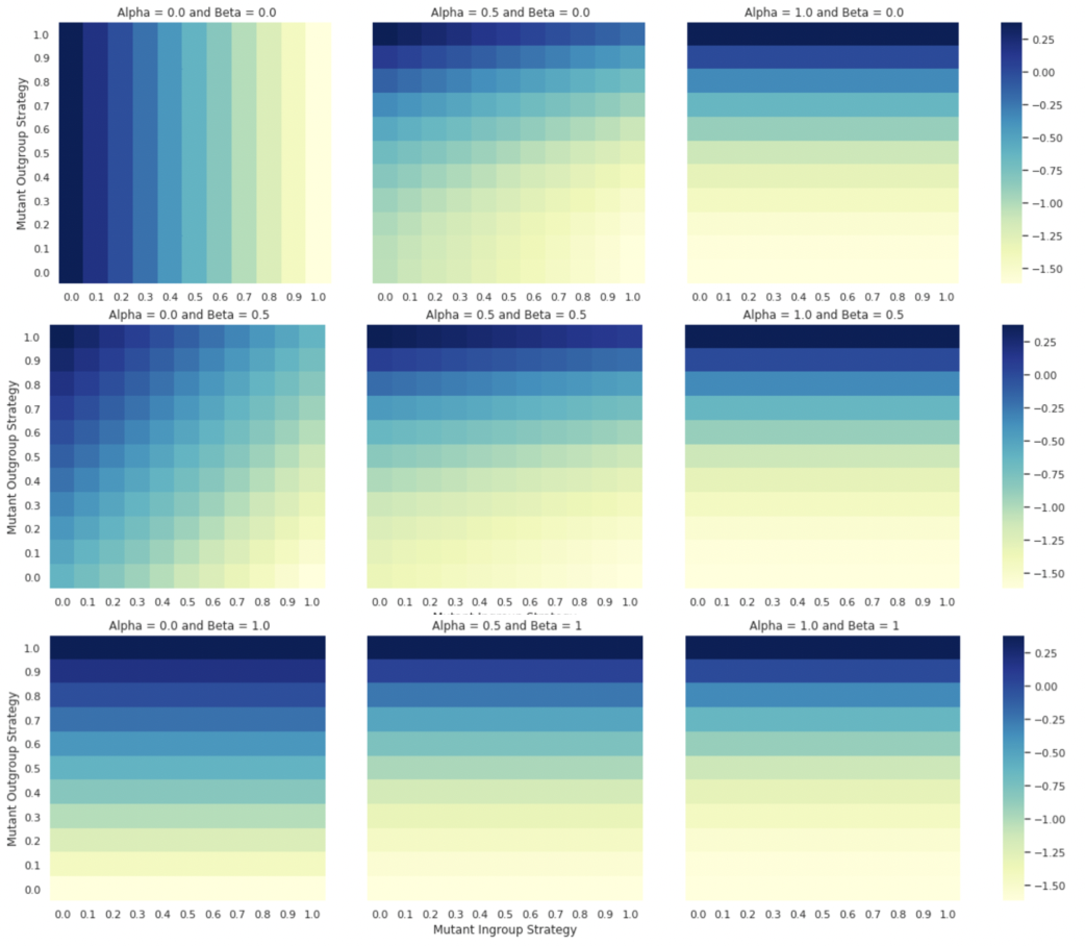
\includegraphics[width=15cm]{images/alpha_beta}
\end{figure}

\section{Model with Alpha, Beta and Delta Parameters}

\subsection{Introduction to Infinitely Repeated Stag Hunt}

Now we extend the model from a once-off stag hunt to an indefinitely repeated stag hunt game. Let delta be the continuation probability of the pair of agents playing an additional round of the game. Therefore, each pair plays at least once but the total number of games each pair plays follows a geometric distribution. Delta is included to model when social encounters are repeated over time when agents meet and to investigate long-term behaviour. 
\\
We extend to the once off model to a repeated model by replacing the once-off payoffs in the payoff matrix with normalised discounted payoffs. 
\\
The normalised discounted rewards are given by 
\[
(1-\delta) \sum_{t=0}^{\infty} \delta^{t}\pi_t 
\]
where $\pi_t$ is the payoff in round t. 
The discounted payoff at either Nash equilibrium when agents both cooperate or defect remains the same since neither agent has incentive to deviate so both agents will continue playing the same strategy and receiving the same payoff for all future time steps.  However, for the other two states, the discounted payoffs equal the immediate payoff of playing that strategy plus the discounted series of most probable future payoffs. In both cases, when the agent cooperates when their opponent defects or the agent defects when their opponent cooperates, the most likely next state will be the risk-dominant Nash equilibrium when both agents defect.  \\
Therefore, the discounted payoff matrix will be 
\[
  \begin{pmatrix} 
   R\frac{1}{1-\delta} & S + P\frac{\delta}{1-\delta}  \\
   T + P\frac{\delta}{1-\delta}  & P\frac{1}{1-\delta} 
   \end{pmatrix} 
\]

and the normalised discounted payoff matrix is given by 

\[
  \begin{pmatrix} 
   R & S(1-\delta) + P\delta  \\
   T(1-\delta) + P\delta  & P
   \end{pmatrix} 
\]


\subsection{Adaptive Dynamics Analysis}

Let $ \Pi ( y, x_{-}, \alpha, \beta_y, \delta)$ be the payoff function of playing a strategy $y = (y_{in}, y_{out}) $ against the dominant strategy $x = (x_{in}, x_{out})$  where $\alpha$ is the probability that an agent is matched to play against a copy of themselves instead of their original opponent, $\beta$ is the probability of an agent playing an individual from the ingroup and $\delta$ is the continuation probability.
\\
$ \Pi ( y, x_{-}, \alpha, \beta_y, \delta)$ is derived following the same procedure as $ \Pi ( y, x_{-}, \alpha, \beta_y)$ by replacing the once-off payoff matrix with the normalised discounted payoff matrix.

The invasion fitness of a mutant strategy y in a population with a dominant strategy x is given by 
\[
f_x(y) = \Pi ( y, x_{-} , \alpha, \beta_y, \delta) - \Pi ( x, x_{-} , \alpha, \beta_x, \delta) 
\]
\begin{multline}
f_x(y) = \alpha (R - (S(1-\delta)+P\delta) -(T(1-\delta)+P\delta)+P) y_{in}^2 + (\alpha(R - (S(1-\delta)+P\delta) \\
-(T(1-\delta)+P\delta)+P) + (1-\alpha)\beta_y((S(1-\delta)+P\delta)-P))y_{in} + (1-\alpha)(1-\beta)((S(1-\delta)+P\delta)-P)y_{out} \\ 
- (\alpha + (1-\alpha)\beta_x)(R - (S(1-\delta)+P\delta) -(T(1-\delta)+P\delta)+P)x_{in}^2 + ((1-\alpha)\beta_y(T-P) - (\alpha+\\(1-\alpha)\beta_x)((S(1-\delta)+P\delta)+t-2P))x_{in} - (1-\alpha)(1-\beta_y)(R - (S(1-\delta)+P\delta) -(T(1-\delta)+P\delta)+P)x_{out}^2 \\+((1-\alpha)(1-\beta_y)(T-P) - (1-\alpha)(1-\beta_x)((S(1-\delta)+P\delta)+T-2P))x_{out} + (1-\alpha)\beta_y(R - (S(1-\delta)+P\delta) -\\(T(1-\delta)+P\delta)+P)x_{in}y_{in} + (1-\alpha)(1-\beta_y)(R - (S(1-\delta)+P\delta) -(T(1-\delta)+P\delta)+P)x_{out}y_{out} + (1-\alpha)P
\end{multline}
The selection gradient and the evolutionarily singular strategies for the complete model are given by
\[
D(x) = \diffp*{f_x(y)}{y}{y=x}
\]
\\
\begin{multline}
D(x) = ((2\alpha + (1-\alpha)\beta_y)(R - (S(1-\delta)+P\delta) -((T(1-\delta)+P\delta)(1-\delta)+P\delta)+ P) x_{in} + \alpha((S(1-\delta)+P\delta)\\+(T(1-\delta)+P\delta)-2P), (1-\alpha)(1-\beta_y)((R - (S(1-\delta)+P\delta) -((T(1-\delta)+P\delta)(1-\delta)+P\delta)+ P) x_{out} \\+ ((S(1-\delta)+P\delta)-P)))
\end{multline}
\[
D(H) = 0
\]
\begin{multline}
H = (\frac{\alpha(-(S(1-\delta)+P\delta)-(T(1-\delta)+P\delta)+2P)}{(2\alpha + (1-\alpha)\beta_y)(R - (S(1-\delta)+P\delta) - (T(1-\delta)+P\delta) + P)},\\ \frac{P-(S(1-\delta)+P\delta)}{(1-\alpha)(1-\beta_y)(R - (S(1-\delta)+P\delta) - (T(1-\delta)+P\delta) +P)}) 
\end{multline}
\\
The selection gradients and evolutionary singular points are different with respect to the ingroup and outgroup strategies as a result of agents playing their ingroup strategies when their opponent is replaced with a copy of themselves. 



\end{document}
